\section{Data Acquisition Pipeline} \label{sec:meth_DataAcquisitionPipeline}

% Discuss aggreement between manual coders

Data gathered from Tobii ET5 is processed through a 3-step pipeline, as illustrated in figure \ref{fig:meth_DataAckPipeline}. This \textit{Data Acquisition Pipeline} is required to go from a raw data stream of eye-tracking data to a dataset ordered by timestamps, labeled, and ready for classification. Each step will be detailed further in the following sections.

\begin{figure}[h]
    \centering
    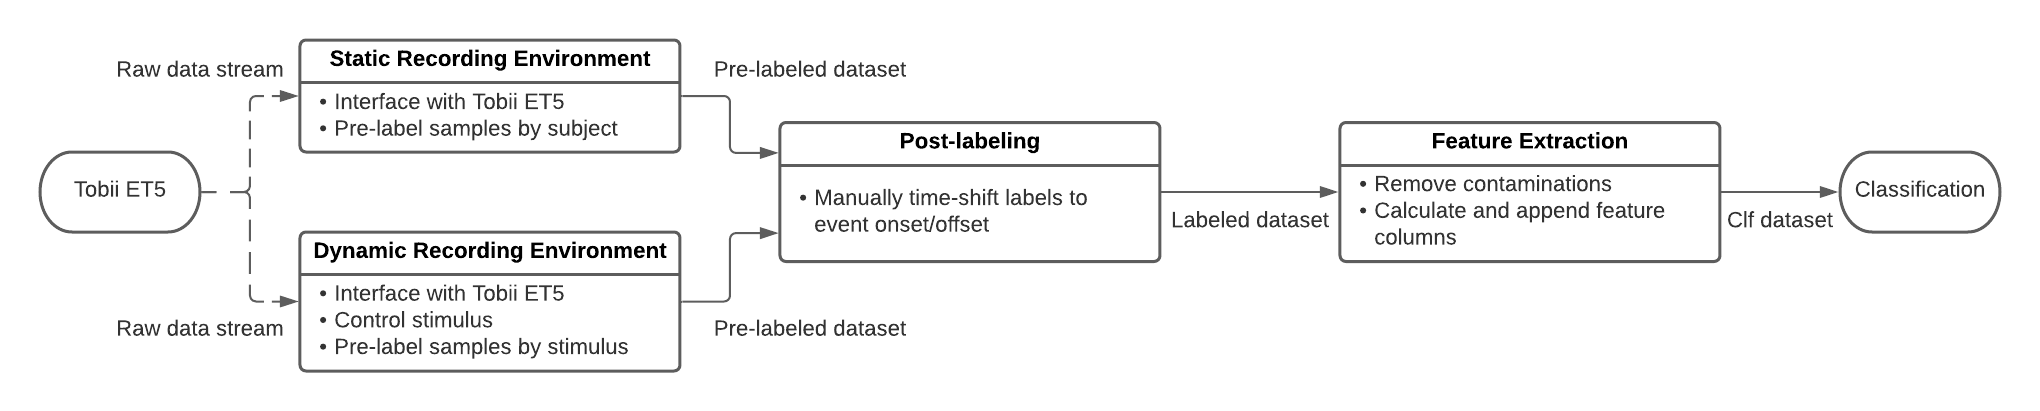
\includegraphics[width=\textwidth]{Images/meth_dataAckPipeline.png}
    \caption{Data Acquisition Pipeline. Each box is a step in the pipeline. Dotted lines are data streams, full lines are datasets.}
    \label{fig:meth_DataAckPipeline}
\end{figure}